\begin{savequote}[75mm]
A new life awaits you in the Off-world colonies! A chance to begin again in a golden land of opportunity and adventure!
\qauthor{Blade Runner}
\end{savequote}

\chapter{A hypermedia model of the user on-line footprint}

\newthought{Web services} use personal data to sustain their business by fuelling this stream of information to recommendation systems to generate tailored advertising. When users decide to subscribe a service, they automatically lose control over the data generated by their activity. This is especially true when third parties are authorised to access a user's profile and information. This is often the case of mobile and web application implementing their log-in flow through a larger authorisation provider, like Google or Facebook. We introduce an hypermedia model of the user on-line footprint and present a privacy broker allowing users to retain control on their data. Our proposal uses the blockchain paradigm and build on it to define an identity management system. Our defined model that can be both used to transfer data between services and clients and to express the value and risk of sharing certain information.

\section{Background}

The business model of many services and applications on today's web is based on having user authenticate and, completely or partially, generate data to \emph{pay} for the possibility to use the service. Data is, in fact, used as a currency that can be resold for a variety of purposes. To target the users and suggest back product that they can buy, or to continuously track them across different visits, and in some cases different devices and websites.

Web services can furthermore dispose of the data collected as their property, as when users access a service they lose control and rights over their digital footprint. One of the problem associated with this is certainly linked to consent. Users give their implicit consent to the use of their data and subsequently their footprint, sometimes only in part, become property of the company providing the services. The same process of giving consent or granting permissions to access part of the user identity is not clear. This scenario is particularly evident when mobile applications request access to some resources on a user's phone, or when Facebook federated log-in mechanism is used. Facebook log-in provides both authentication and authorisation. The mechanism is used on the web as well as on iOS and Android, although on those platforms the primary mechanism uses the native Facebook application instead of the web API. When an application is connected to the user's Facebook profile using Facebook log-in, it can always access their \emph{public profile} information. Facebook consider this information public and will not apply any restriction on it. Information that is shared with the public profile vary from user to user and depends on their privacy settings. By default the Facebook public profile includes some basic attributes about the person such as the user's age range, language and country, but also the name, gender, username and user ID (account number), profile picture, cover photo and networks. This is the minimum set of data disclosed by Facebook when the social network log-in mechanism is used to gain access to an app or service. This data is acquired by the app and user control over it is practically lost, as it will be disposed according to the app privacy policy.

We propose a model of the user identity and a privacy management system based on the OAuth 2.0 flow which uses JWT to transmit private information to third parties. This approach is similar, and builds upon, previous techniques, such as Crypto-Book~\cite{maheswaran2013crypto} and UnlimitID~\cite{isaakidis2016unlimitid}, using the technique of blacklistable anonymous credentials. We would like to stress that no modification is needed for existing web protocols or clients and that we make use of existing and widely adopted authorisation and authentication mechanism. Furthermore, the proposed hypermedia model allows the user to explore the shared preferences and properties shared with each service.

\section{A hypermedia model of the user identity}

Users interact with web services and applications with hypermedia protocols. Each time an action is completed onto an user's phone a call is performed to an APIs updating the user profile or sending some information to a service. These interactions are often completed over a REST protocol, such as HTTP, and consist of the client (in this case the user phone) sending structured information to the server (in this case the app backend). This information can be anything regarding the user or the state of the used application, such as profile information or answers to specific queries initiated implicitly or explicitly by the user.

We define a model of the user identity to describe how a privacy policy can interact with data and which data or resource a service can access. Our model is based on the assumption that user data can be represented with a hypermedia object. This specifically mean that accessing a resource at a given time or accessing identification information opens up access to data connected to that resource or that identification. We begin by defining the identity model using JSONApi~\cite{Jsonapi} a specification for exchanging data between REST interfaces defining how a client should request that resources or their representations be fetched or modified, and how a server should respond to those requests. We envision that the same format can be used on the client side to represent identities and data associated with it and on the server side to request and exchange data.

\begin{lstlisting}
{
    "data": {
        "type": "identity",
        "id": "john@johnsmith.com",
        "attributes":
            { // Attribute list },
        "relationships":
                { // Relationship list },
        "links": { // Third-party links }
    },
    "included": [ {
        "type": "resource",
        "id": "CC76598TDZKG9EEC3", // Device hardware id
        "attributes": { // resource attributes }
        "meta": { // Any meta information },
    }],
}
\end{lstlisting}

We model the user's activity as series of events belonging to a certain identity. Each event is a document containing different information. We can formally defined this an hypermedia document i.e. an object possibly containing graphics, audio, video, plain text and hyperlinks. We call the hyperlinks selectors and we use these to build the connections between the user's different identities or events. Each identity is a profile that the user has created onto a service or platform. This can be an application account or a social network account, such as their LinkedIn or Facebook unique IDs.

Each event is the result of the user performing an action. For the purpose of this study we have consider an action as resulting using an application or a service. An action is the activity of interacting with a mobile application or \emph{liking} a resource on a social network, i.e. directly expressing an interest, or the fact that a user has updated their location at a certain time.

We find that this model is able to express the user's on-line footprint as a collection of traces left across different services. Furthermore by using a hypermedia approach we are able to grasp the connections between the different profiles and features. This results in the possibility to profile users based on chosen selectors. For example we might want to trace all users who have been in the radius of 500 meters to a certain location, or all the users in a certain neighbourhood who \emph{like} a selected Facebook page.

\section{Proposing a privacy management system}

We now propose a privacy management system that would be able to give users more control over their data and desired footprint, given the hypermedia model proposed above. Our system is based on the widely adopted oauth 2.0 protocol~\cite{hardt2012oauth} for authorisation and uses signed and JSON Web Token (JWT)~\cite{jones2015json} Bearer Token as a means for requesting an access token as well as for client authentication.

The abstract OAuth 2.0 flow describes the interactions between different parties (Figure: ~\ref{fig:oauth2flow}). These are:

\begin{itemize}
    \item Client
    \item Resource Owner
    \item Authorisation Server
    \item Resource Server
\end{itemize}

\begin{figure}
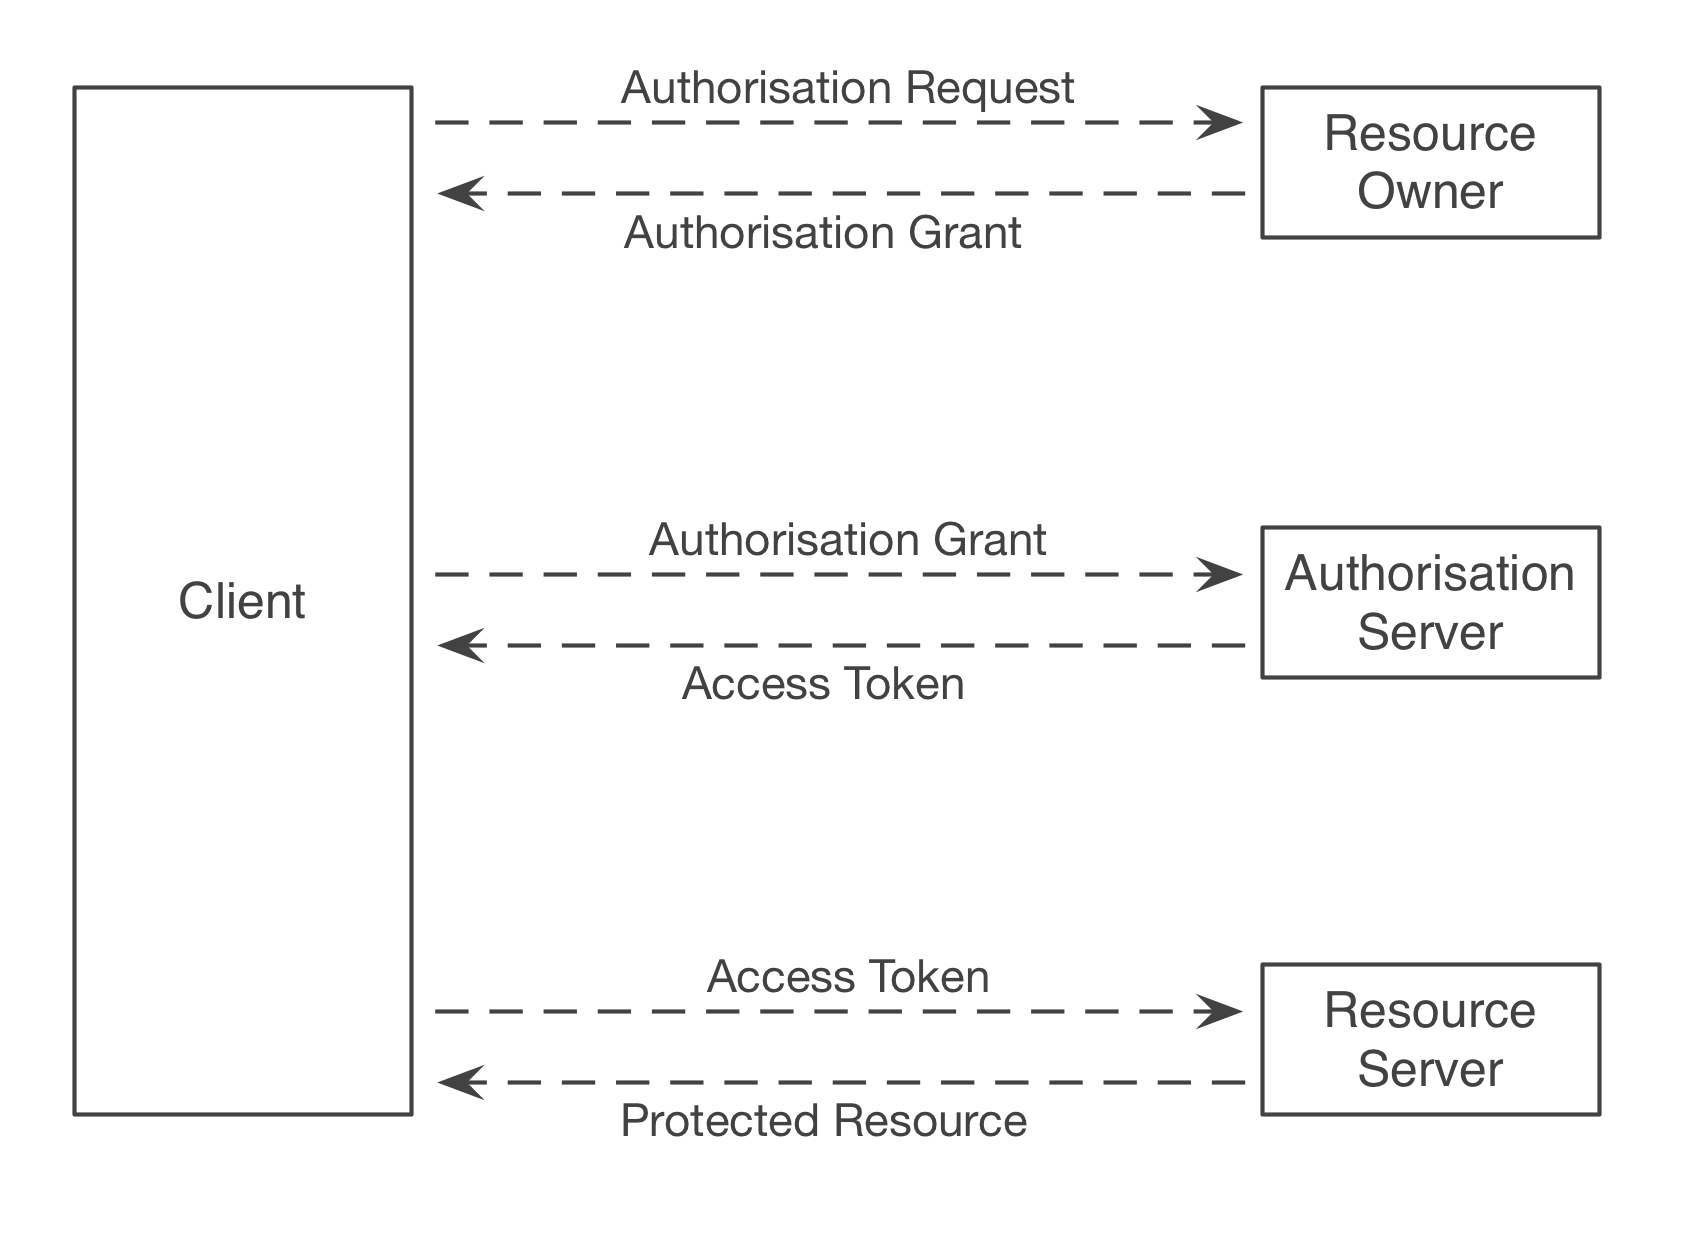
\includegraphics[width=\textwidth]{figures/OAuth2Flow.png}
\caption[OAuth 2.0 Flow.]{The abstract OAuth 2.0 flow describes the interaction between the four roles within the defined steps.
\label{fig:oauth2flow}}
\end{figure}

The six steps in the abstract OAuth 2.0 flow are defined as follows:
\begin{enumerate}
    \item The client sends an authorisation request to the resource owner, either directly or via the authorisation server as intermediary.
    \item The client receives an authorisation grant.
    \item The client requests an access token by presenting the authorisation grant.
    \item The client is authenticated by the authorisation server which issues and access token.
    \item The client now requests the protected resource presenting the access token.
    \item The resource server validates the token and replies with the resource representation if valid.
\end{enumerate}

JSON Web Token (JWT)~\cite{jones2015json} is a compact, URL-safe mechanism to represent and transfer claims between two parties. The claims are encoded as a JSON object. This can be used as the payload of a JSON Web Signature (JWS)~\cite{jones2014n} structure, or as the plaintext in a JSON Web Encryption~\cite{jones2015jwe} structure. Therefore, JWT allows for the claims to be digitally signed or integrity protected integrity protected with a Message Authentication Code (MAC) and/or encrypted.

\subsection{Scenario}

We consider a scenario in which a user wants to log-in to a service without having to directly expose their identity, by leveraging with an Identity Provider (IdP). In this scenario we have three parties:
\begin{itemize}
    \item client
    \item service
    \item identity provider
\end{itemize}

The four steps in this OAuth flow are defined as follow (Figure: ~\ref{fig:privateflow}):
\begin{enumerate}
    \item The client sends an authorisation request to the IdP. This request is signed and encrypted and packed into a JWT.
    \item If the request is valid the IdP issues a token.
    \item The client uses the token to authenticate with the service. Which is verified separately with the IdP.
    \item The service returns access to the protected resource through its representation.
\end{enumerate}

\begin{figure}
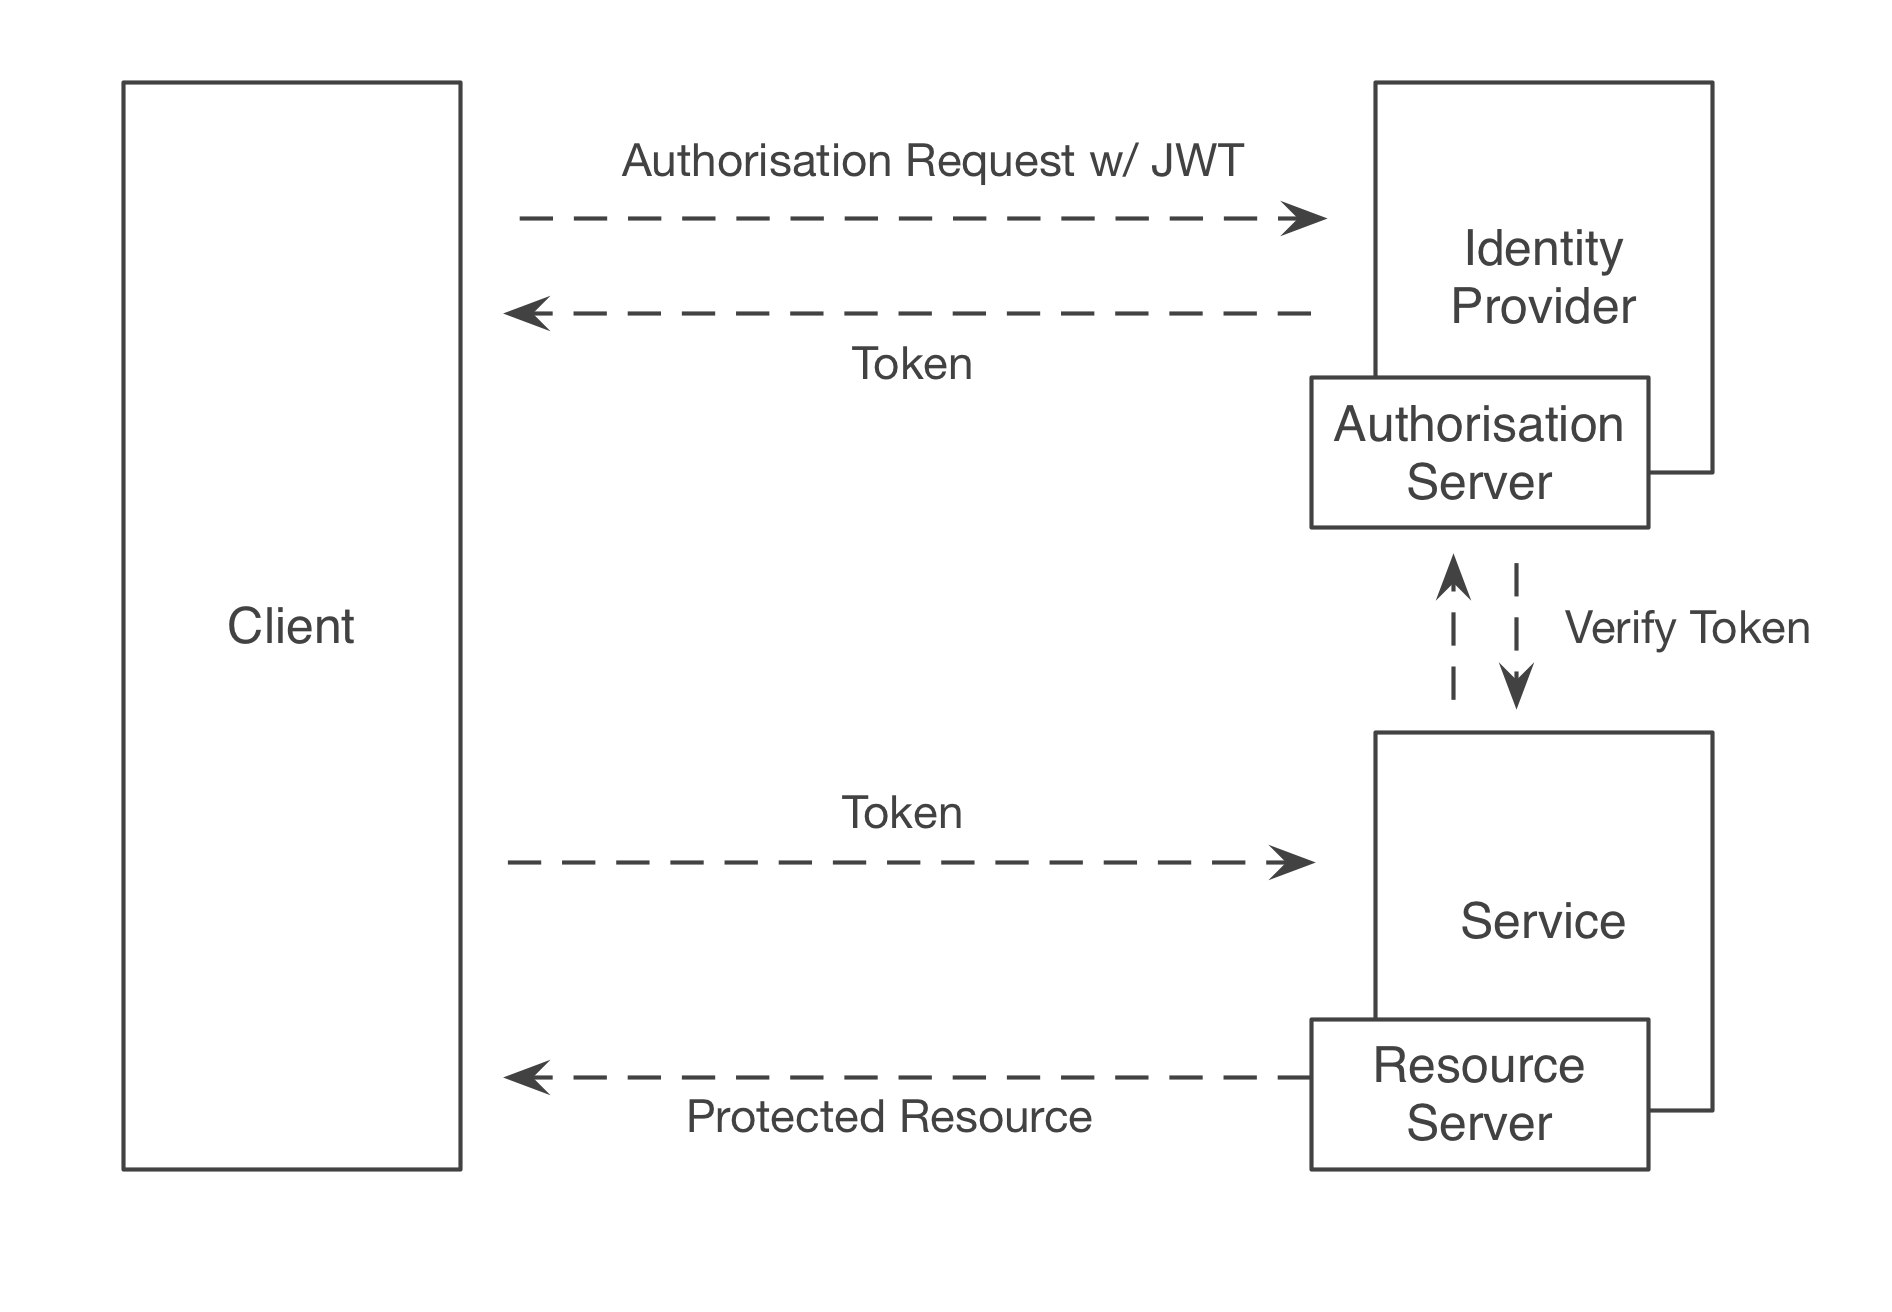
\includegraphics[width=\textwidth]{figures/PrivateFlow.png}
\caption[Privacy Preserving OAuth Flow with JWT.]{The privacy preserving OAuth 2 flow uses JWT to transmit user information.
\label{fig:privateflow}}
\end{figure}

\subsection{Account creation on the IdP}

To create an account on the IdP we assume that as the client is initialised it will generate a number of cryptographic keys to authenticate the various user identities. The keys can be saved in a wallet and used to register identities on the IdP. A use might decide to use different keys for each service or the same key for a group of services. Note that each key doesn't correspond to a service account Id. A key is actually an account identification for the IdP which is stored and used by the client.

To create an account on a service the client prepares a request for the IdP performing a set of cryptographic operations that allows the client to register an anonymous identifier for the service. To implement such algorithm we need a
cryptographically secure hash function and a secure elliptic curve group. JSON Web Algorithms (JWA)~\cite{jones2015jwa}, provides Hash-based Message Authentication Codes (HMACs). HMACs enable the client to compute a MAC from a secret (the user's key) plus a cryptographic hash function. The algorithm for implementing and validating HMACs is provided in RFC 2104~\cite{krawczyk1997rfc}.

\subsection{Authorisation request}

Once the client is issued a \emph{token} from the IdP it can authenticate with the \emph{service}. Hence, the issued \emph{token} which encodes the claims and service id can be transmitted to the service encrypted with the JWE protocol. The token can then be verified and the client authorised to request the protected resource. An account is created on the service if the authentication protocol is initiated for the first time.

\subsection{Protocol Flow}

The protocol flow was implemented as follows:
\begin{enumerate}
    \item The client sends an authorisation request to the IdP.
    \item The client receives an authorisation grant via a \emph{JWT} encoding the 0-knowledge proof to present to the SP.
    \item The client engages the SP in a zero-knowledge proof that it holds a valid credential from the IdP.
    \item The client is authenticated (or not).
    \item The client can now request protected resources, or the SP can request further information from the client.
\end{enumerate}

-- begin comments --

JWT implementation.
Which fields are used, how.
Which fields are transmitted in third-party authentication mechanism w/ facebook? How would this change?
How would this affect the information shared from the client?
Also with the current model third-party apps might request access to all entities the user has created or has interacted with (Posts, pages liked) now the user might instead share only a profile that has been sanitised before hand ---> Tag forgery/Tag suppression/ Share a uniform profile/ no preferences expressed.

-- end comments --

\section{Privacy Management}

The protocol flow described up to this point allows the client to granularly disclose information to the SP. More importantly in the current federated login mechanism, implemented by IdPs like Facebook, third-party apps can always request to the IdP updated information regarding the user. With the proposed mechanism, third-party apps will have to request the information to the client, that can refuse to provide them or can provide different values depending on the context.

-- begin comments --

Properties of the protocol. Unlinkability ... what else?
Can be used in anonymous communication systems preserving user anonymity while at the same time preventing 

-- end comments --

\section{Prototype Evaluation}

Ruby implementation of oauth2 with JWT.

\section{Discussion}
